\documentclass[../../memoria.tex]{subfiles}

\begin{document}

\begin{figure}[H]
    \centering
    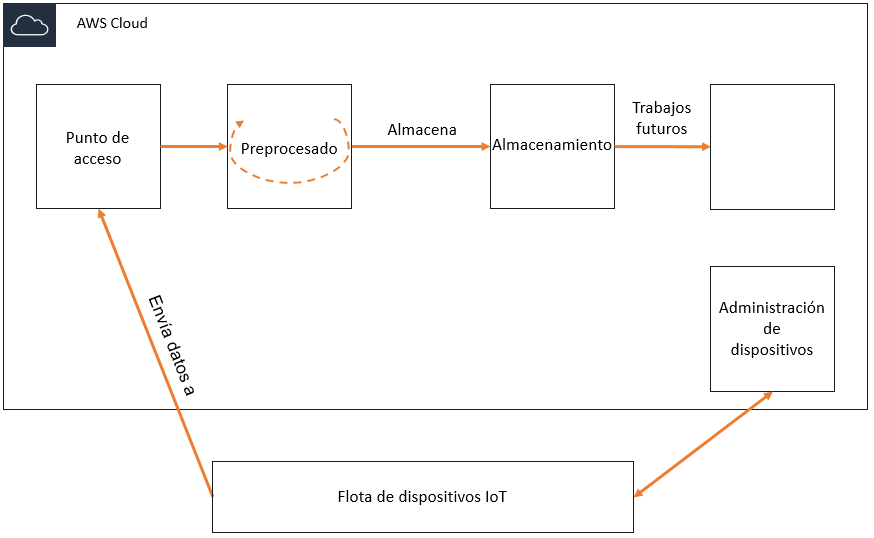
\includegraphics[width=0.7\columnwidth]{figura1.png}
    \caption{Esqueleto del escenario básico}
    \label{fig:figura1}
\end{figure}

\paragraph{}
Como puede observarse en la Figura 1, la idea principal es dar una solución para los elementos punto de acceso, preprocesado y almacenamiento, que esté implementada de tal manera que sea compatible con cualquier elemento que se establezca como la flota de dispositivos IoT y trabajos futuros. Asimismo, establecer un sistema de administración de dispositivos con una comunicación bidireccional para trabajos de actualización o monitorización del propio dispositivo IoT.

\paragraph{}
Un ejemplo de implementación para la flota de dispositivos IoT sería lo que se puede apreciar en la siguiente imagen:

\begin{figure}[H]
    \centering
    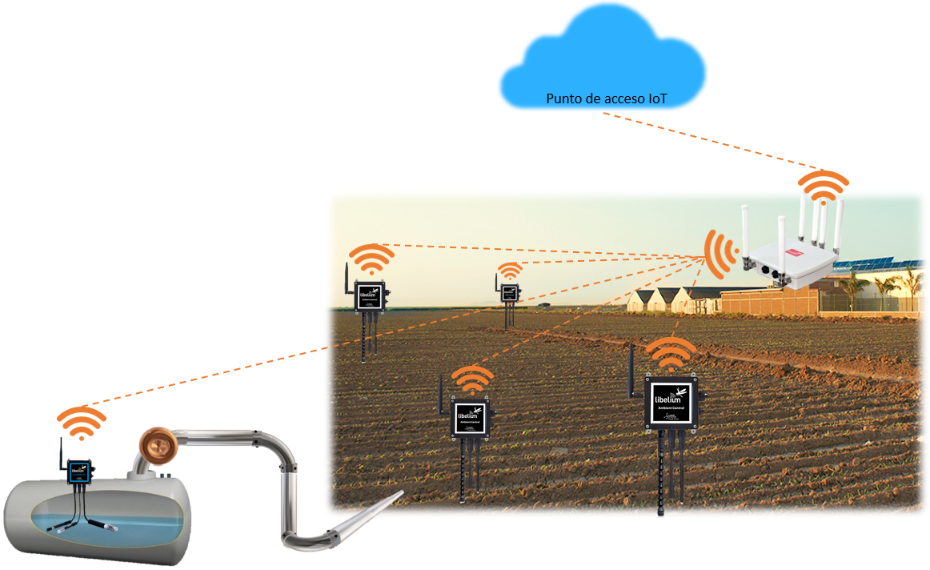
\includegraphics[width=0.7\columnwidth]{figura2.png}
    \caption{Ejemplo de flota de dispositivos IoT para una tierra de cultivo.}
    \label{fig:figura2}
\end{figure}

\paragraph{}
En la Figura 2, pueden verse diferentes dispositivos del fabricante Libelium, en concreto están ubicados como sensores diferentes modelos Plug \& Sense! de Libelium: Ambient Control en la tierra y Smart Water en el depósito de agua. También, como punto centralizado de los sensores y punto de conexión con Internet, se encuentra en las naves instalado un dispositivo Meshlium Xtreme que actúa como IoT \textit{Gateway} \cite{libelium}. Como punto de entrada al sistema en \textit{Cloud}, el Meshlium Xtreme comunicaría los datos recogidos al punto de acceso, el cual correspondería con el mostrado en la Figura 1. Esto es simplemente un ejemplo teórico de una solución que sería compatible con el sistema que se pretende implementar con este proyecto.

\paragraph{}
Por lo tanto y como primer sistema se va a desarrollar el siguiente escenario, utilizando el IoT Core de AWS, el servicio de computación AWS Lambda y el Elasticsearch Service.

\begin{figure}[H]
    \centering
    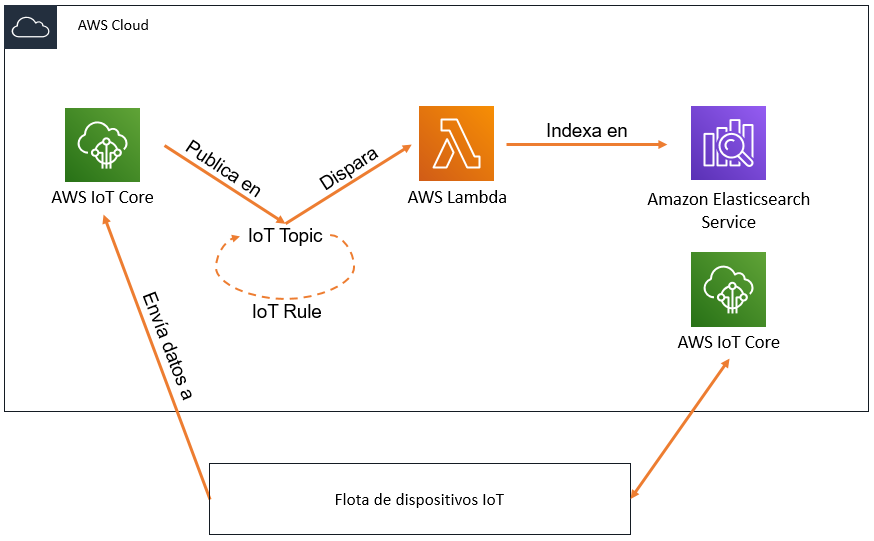
\includegraphics[width=0.7\columnwidth]{figura3.png}
    \caption{Ejemplo del escenario base del sistema.}
    \label{fig:figura3}
\end{figure}

\paragraph{}
En la Figura 3 se pueden ver los diferentes elementos del sistema a los que se les ha dado una respuesta utilizando diferentes servicios de AWS. A grandes rasgos, el funcionamiento del sistema es el siguiente:

\begin{enumerate}
    \item La flota de dispositivos IoT envía información a un punto de acceso situado dentro del servicio IoT Core de AWS. En concreto, se enviará la información a un IoT Topic, el cual no es más que una implementación del protocolo MQTT \cite{mqtt}. Por tanto, el elemento que envíe hacia el Topic únicamente tendrá que implementar un cliente MQTT para enviar los datos (más adelante se hablará sobre cómo se implementa de manera segura esta conexión).

    \item Al recibir un mensaje en el Topic de IoT, una IoT Rule del servicio IoT Core de AWS se encargará de realizar una acción con dicho mensaje. En este ejemplo, ese mensaje se envía como entrada a una función desplegada en el servicio AWS Lambda (más adelante se explicará la razón de utilizar una función como intermediario y no utilizar la acción por defecto que ofrece la IoT Rule para indexar en Elasticsearch Service).

    \item Mediante la función Lambda, se realiza un preprocesado de los datos recibidos y se indexa en el servicio Elasticsearch Service, que actúa como base de datos.

    \item Una vez almacenados los datos en la base de datos de Elasticsearch Service, se pueden lanzar las consultas que sean necesarias para obtener los datos que se requieran, o puede configurarse el motor de visualización que viene incluido por defecto en el servicio, Kibana, para representar los datos indexados como desee el usuario. Este último punto pertenece al elemento trabajos futuros representado en el esqueleto del sistema de la Figura 1.
\end{enumerate}

\paragraph{}
A continuación, se presenta un análisis detallado del sistema y de las razones de usar los servicios mencionados:

\begin{itemize}
    \item En primer lugar, con respecto al IoT Topic del AWS IoT Core, se ha utilizado ya que se necesita únicamente un cliente de MQTT desde la parte Hardware del sistema. Es un protocolo altamente extendido y muy liviano, que encaja a la perfección en un sistema IoT de estas características. Por lo tanto, este IoT Topic se presenta como una cola MQTT a la que se publica apuntando hacia un \textit{endpoint}, que es global para toda la cuenta en AWS, y especificando el nombre del IoT Topic. Además, para que esta conexión sea segura, desde el IoT Core, se pueden registrar dispositivos haciendo uso de certificados. Para registrar un dispositivo, se generará un certificado mediante el cual se identificará dicho dispositivo para enviar los datos. De esta manera se realiza la comunicación de manera segura, y el punto de acceso no estará habilitado a cualquier fuente, sino que, mediante una política de seguridad, únicamente se podrán enviar datos desde los dispositivos registrados.

    \item En segundo lugar, haciendo alusión al tercer punto del funcionamiento del sistema anteriormente presentado, se utiliza un intermediario entre el IoT Core y el Elasticsearch Service. Desde una IoT Rule, es posible indexar de manera directa en un Elasticsearch Service desplegado, pero se ha decidido introducir una función Lambda que haga de intermediario debido a la necesidad de compatibilidad con todo tipo de sistemas. De este modo, se produce un desacoplamiento entre ambas capas del sistema, lo que permitiría la adaptación a otros requerimientos modificando únicamente la función Lambda y no parte del servicio de IoT Core. Operacionalmente es mucho más sencillo redesplegar una Lambda mediante Terraform, que modificar la configuración interna del IoT Core y de la IoT Rule. Además, una función Lambda permite un grado de libertad sobre el procesamiento e indexado de los datos mucho mayor que permitirá adecuarse mucho más a las especificaciones concretas del sistema. Además, si por ejemplo surgiese la necesidad de cambiar Elasticsearch Service por una instalación del Stack de Elastic sobre instancias EC2, obligaría a cambiar la configuración del IoT Core mientras que usando esta Lambda únicamente sería necesario cambiar el punto de acceso a Elasticsearch.

    \item Por último, este sistema está enteramente basado en la computación \textit{serverless}. La computación \textit{serverless} se basa en utilizar servicios gestionados por un proveedor para que el usuario no tenga que desplegar y administrar sistemas o servidores. Normalmente se ofrecen como servicios con un precio mayor al que supondría montar el mismo sistema utilizando máquinas virtuales o instancias, pero se eliminan los costes operacionales de dicha instalación \cite{awsserverless}. Para un proyecto de este tipo, este tipo de computación ofrece la posibilidad de utilizar servicios difíciles de instalar y mantener, de manera sencilla por cualquier usuario no experimentado. Es por ello que para este proyecto se ha optado por seguir esta filosofía para la totalidad del proyecto, pudiendo intercambiar los diferentes elementos mencionados en la Figura 1 por componentes más tradicionales implementados sobre una máquina virtual o un servidor. Elasticsearch Service se ofrece como un servicio gestionado, dentro de la computación \textit{serverless}. Utilizar un servicio gestionado permite no tener que administrar ningún tipo de servidor. Además, usar Elasticsearch permitirá en los trabajos futuro utilizar su propio motor de búsqueda para lanzar consultas a su base de datos, por lo que no será necesario un motor de búsqueda adicional. Esto sigue en la línea de buscar la mayor compatibilidad posible con otros elementos que se añadan al sistema. A modo de ejemplo, podría instalarse el Stack de Elastic sobre instancias EC2 y llevar a cabo la instalación de este en la duración de este proyecto, sin embargo, se ha considerado más interesante dedicar mayor cantidad de tiempo al sistema en general que a la instalación de sus diferentes elementos. Es por ello por lo que se ha optado por usar este tipo de computación \textit{serverless}.
\end{itemize}

\end{document}
